\section{Metacognitive Alignment and Availability Readouts}
\label{sec:extensions}

\begin{table}[t]
\centering
\caption{\textbf{Metacognitive alignment}, two model families: ${\sim}$500
fine-tuning steps on yes/no labels derived from each model's own workspace
ranking, using disjoint benchmarks (Evoked, Explicit, Evoked-G2). The verbal
channel is repaired on fully held-out benchmarks (+0.28--0.39 AUC) while the
workspace channel is untouched, full-context QA is statistically unchanged,
and general capability (MMLU, GSM8K, ARC) is unaffected (Table~\ref{tab:geneval})
(App.~\ref{app:metacog}). For the Qwen-0.5B Compositional row the repaired
reporter converges to its teacher's (chance) level; where generation-time
computation adds signal (OLMo Compositional) the student can exceed the
static teacher (\S\ref{sec:metacog}).}
\label{tab:metacog}
\small
\resizebox{\textwidth}{!}{%
\begin{tabular}{llcccc}
\toprule
\multirow{2}{*}{Model} & \multirow{2}{*}{Held-out benchmark} & \multicolumn{2}{c}{Verbal report $V$ (AUC)} & \multicolumn{2}{c}{Workspace $W$} \\
\cmidrule(lr){3-4} \cmidrule(lr){5-6}
 & & before & after & before & after \\
\midrule
OLMo-2-1B & Decoupled & 0.326 [0.251, 0.400] & \textbf{0.671}\dgain{+0.35} [0.584, 0.751] & 0.580 & 0.586 \\
OLMo-2-1B & Compositional & 0.267 [0.179, 0.360] & \textbf{0.580}\dgain{+0.31} [0.482, 0.677] & 0.477 & 0.491 \\
\addlinespace
Qwen2.5-0.5B & Decoupled & 0.281 [0.210, 0.354] & \textbf{0.668}\dgain{+0.39} [0.595, 0.737] & 0.526 & 0.524 \\
Qwen2.5-0.5B & Compositional & 0.172 [0.112, 0.241] & \textbf{0.451}\dgain{+0.28} [0.367, 0.534] & 0.416 & 0.409 \\
\bottomrule
\end{tabular}
}
\end{table}


\begin{figure}[t]
\centering
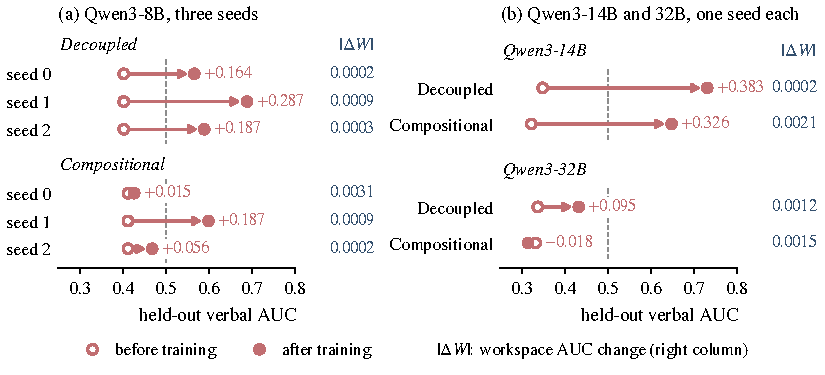
\includegraphics[width=0.95\textwidth]{figures/fig4_development_repair.pdf}
\caption{\textbf{Post-training changes the verbal channel, not the workspace
channel, and the verbal channel is repairable.} \textbf{(a)}~OLMo-2-1B released post-training stages: the
workspace channel ($W$, blue) never improves from base, on either benchmark, while
the verbal channel ($V$, rose) stays at chance (Evoked) or far below it
(Compositional). \textbf{(b)}~Metacognitive alignment: ${\sim}500$ self-distillation
steps move the verbal channel (arrows) from below-chance to well-calibrated on fully
held-out benchmarks while leaving the workspace channel in place (open circle =
before, filled = after).}
\label{fig:devrepair}
\end{figure}

\subsection{Metacognitive Alignment}
\label{sec:metacog}

If the model knows more than it tells because telling was never trained
against the knowing (Fig.~\ref{fig:devrepair}), the reporter should be
trainable from the model's own workspace signal, without human annotation. We fine-tune OLMo-2-1B-Instruct for ${\sim}500$ steps on
the exact importance-probe prompt, with yes/no targets derived from the model's
own workspace ranking (top-2 items per episode), using only the explicit and
evoked benchmarks plus the second-generator benchmark (Evoked-G2, gpt-4o); the decoupled benchmarks
(Decoupled, Compositional) are never seen. Table~\ref{tab:metacog} (seed-0 runs; three-seed means $0.62$--$0.65$,
App.~\ref{app:metacog}): held-out verbal calibration jumps from $0.326$ to
$0.671$ and from $0.267$ to $0.580$. The same procedure,
unchanged, replicates in a second family: Qwen2.5-0.5B-Instruct rises from
$0.281$ to $0.668$ (Decoupled) and $0.172$ to $0.451$ (Compositional).
Three controls secure the interpretation: label-shuffled fine-tunes leave
held-out calibration at chance in both families ($0.416$/$0.382$),
distilling from embedding-derived labels fails ($0.458$), and the aligned
reporter rejects context-absent foils ($0.900$), so the gain is specifically
the workspace signal, not format de-biasing, generic salience, or an absence
shortcut (App.~\ref{app:metacog}). The two Compositional endpoints then fit one
prediction: distillation transfers the monitor's signal, so where the static
teacher is at chance (Qwen-0.5B) the student plateaus there, while where
generation-time computation adds signal beyond the static snapshot (OLMo-1B)
the student can exceed the static value, behaving like the dynamic readouts
of \S\ref{sec:family}. The calibration
transfers across held-out benchmarks and generators, which is consistent with the
reporter acquiring a benchmark-independent readout of internal state; shared
construction biases across generators cannot be fully excluded. The workspace channel itself is untouched, and
full-context QA never moves significantly ($-0.029$ for OLMo, $+0/-2$,
$p{=}0.50$; $-0.044$ for Qwen, $+5/-8$, $p{=}0.58$; App.~\ref{app:metacog}). Practically, twenty minutes of self-supervised fine-tuning on one GPU repairs
a channel that SFT, DPO, and RLVR left miscalibrated.

\subsection{A Family of Availability Readouts}
\label{sec:family}

\begin{table}[t]
\centering
\caption{Availability readouts by provenance regime, Qwen-7B AUC.
Full grids and confidence intervals are in App.~\ref{app:family}.
The paired Compositional contrast is $W_J{-}W$: $+0.125$
[$+0.010$, $+0.244$]; App.~\ref{app:vrobust} gives the
conditional-likelihood comparison. Bold marks the column best.}
\label{tab:family}
\small
\begin{tabular}{lccc}
\toprule
Member & Evoked & Decoupled & Compositional \\
\midrule
Spotlight $W$ (static) & 0.633 & \textcolor{gain}{\textbf{0.641}} & 0.514 \\
Broadcast breadth (static) & 0.637 & 0.557 & 0.486 \\
Rehearsal $W_{rep}$ (dynamic) & \textcolor{gain}{\textbf{0.684}} & 0.578 & 0.553 \\
Leverage $W_{J}$ (dynamic) & 0.506 & 0.550 & \textcolor{gain}{\textbf{0.639}} \\
\bottomrule
\end{tabular}
\end{table}


Availability to downstream computation can be operationalized in more than one
way. We evaluate four readouts of the same frozen model: \emph{Spotlight}
($\Wrr$, instantaneous decodability), \emph{Broadcast} (its spatial spread across
positions, in the spirit of global-workspace ignition, \citealp{dehaene2011}),
\emph{Rehearsal} ($W_{rep}$: reactivation across $K$ sampled probe-blind
continuations, an analogue of offline replay), and Leverage ($W_J$: the
directional
derivative of expected future answering utility along the concept's input-side
direction, the infinitesimal form of the causal intervention in
\S\ref{sec:causal}, computed by backpropagation without training: one
forward-plus-backward pass per episode--question pair, with every candidate
scored from the same gradient). The expectation $\mathbb{E}_q$ is over a fixed
bank of 12 probe-blind questions per episode, scored on the model's own greedy
answers $\hat a_q$.
Table~\ref{tab:family} shows a clean double dissociation between readouts:
decode-based members own the evoked regime (Rehearsal reaches $0.684$ on Evoked,
improving on Spotlight), while Leverage is the only member that recovers
compositional bridges under the paired criterion of \S\ref{sec:boundary}
(Compositional at 7B: $0.639$; paired over Spotlight $+0.125$
$[+0.010, +0.244]$, CI excluding zero), at the cost of low sensitivity where decoding is easy. Rehearsal's Compositional
ceiling ($\approx 0.55$) does not move with rollout budget: free-running
generation rarely performs the composition spontaneously, whereas the gradient
detects the latent structure without requiring it to run. Boundaries: the Leverage result does not
replicate on OLMo-2-7B ($0.515$); head-to-head against the
conditional-likelihood baseline on Compositional the two do not separate
($W_J{-}$LL $+0.046$ $[-0.056, +0.153]$, App.~\ref{app:vrobust}), so the
claim is that Leverage is the only \emph{workspace} readout whose paired
gain over the static member is significant, not that it beats every
non-workspace score; and naive member ensembles do not beat the
per-regime best member (App.~\ref{app:family}); availability estimation is regime- and family-dependent, and the dissociation
between readouts parallels, at a lower level, the report--computation
dissociation that motivates this work.
